% Prova del 14/09/2021, esercizio 2 (B65-E02): corrente a M = 5 e incidenza 11° su un corpo piano con un
% segmento sottile davanti; forza sul segmento. Numeri e figure: calcoli.py (stessa cartella).

\documentclass[11pt,a4paper]{article}

\usepackage[T1]{fontenc}
\usepackage[utf8]{inputenc}
\usepackage[italian]{babel}
\usepackage{amsmath,amssymb}
\usepackage[a4paper,margin=2.4cm]{geometry}
\usepackage{array}
\usepackage{siunitx}
\usepackage{booktabs}
\usepackage{graphicx}
\usepackage{float}
\usepackage{hyperref}

\hypersetup{hidelinks}
\setlength{\parindent}{0pt}
\setlength{\parskip}{4pt}
\allowdisplaybreaks
\graphicspath{{figure/}}
\sisetup{output-decimal-marker={,}, group-separator={\,}, per-mode=symbol,
         exponent-product=\cdot, range-phrase={\text{--}}}

\newcommand{\Cp}{C^{+}}
\newcommand{\Cm}{C^{-}}

\title{Gasdinamica -- Prova del 14/09/2021, esercizio 2\\[2pt]
\large Forza sul segmento sottile davanti a un corpo piano}
\author{}
\date{}

\begin{document}
\maketitle

\section*{Traccia}
Una corrente supersonica stazionaria a Mach $=5$ e angolo di incidenza $\alpha=\ang{11}$ investe un corpo piano
($b=0{,}38876$ e $h=1$). Calcolare la forza che agisce sul segmento $h$ (assumere il suo spessore nullo).

\begin{figure}[H]
  \centering
  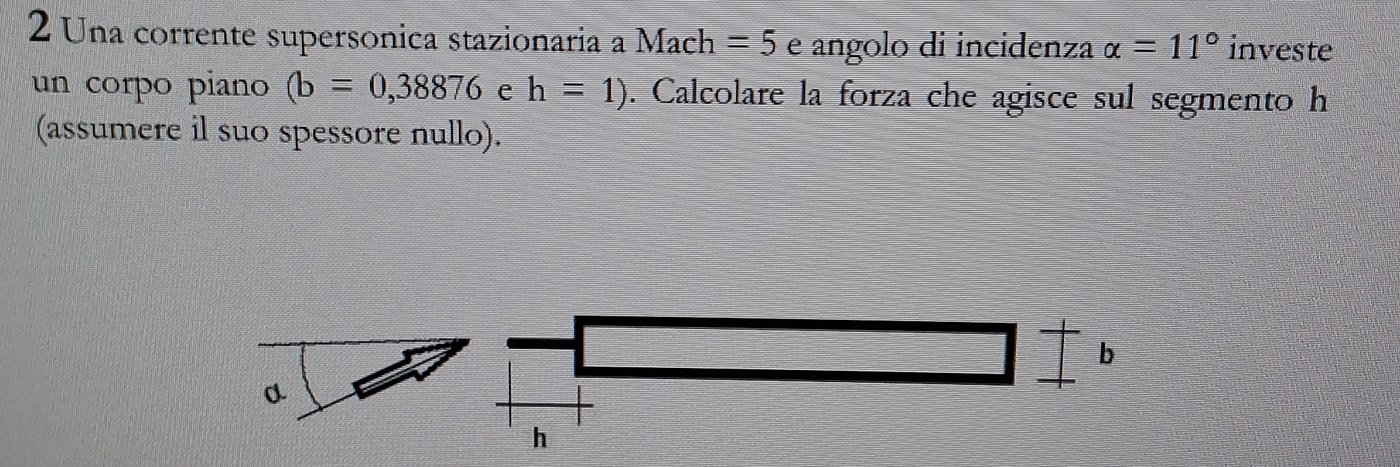
\includegraphics[width=0.8\textwidth]{originale.png}
  \caption{Traccia originale.}
\end{figure}

%==============================================================================
\section{Lettura del testo e dati}
Il corpo è formato da un segmento sottile di lunghezza $h$, rivolto verso la corrente, attaccato alla faccia
anteriore di un corpo rettangolare di altezza $b$. La corrente arriva da sotto, inclinata di $\alpha=\ang{11}$ sul
segmento. Si chiede la forza sul solo segmento, cioè la differenza fra le pressioni sulle sue due facce per la sua
lunghezza: serve sapere quale pressione ``vede'' ciascuna faccia.

Il dato $b$ è dato con cinque cifre, ed è il primo indizio:
\[
\frac{b}{2h}=0{,}19438=\tan\ang{11}=\tan\alpha .
\]
Le rette che congiungono lo spigolo d'attacco O del segmento con gli spigoli anteriori del corpo sono inclinate
esattamente di $\pm\alpha$, purché il segmento sia in mezzeria. Il disegno non è in scala ($b/h$ disegnato vale circa
0,8) e mostra il segmento circa a metà altezza: assumo che sia esattamente in mezzeria, come suggerisce questa
coincidenza.

Interpretazioni:
\begin{itemize}
\item ``corpo piano'': corrente piana, forza per unità di apertura;
\item gas: aria, $\gamma=1{,}4$ (non indicato);
\item stato a monte non assegnato: pressioni riferite a $p_1$, forze a $p_1h$ e alla pressione dinamica
  $q_1=\tfrac12\rho_1V_1^2=\tfrac{\gamma}{2}p_1M_1^2=17{,}5\,p_1$.
\end{itemize}

\begin{table}[H]
  \centering
  \begin{tabular}{lll}
    \toprule
    Grandezza & Valore & Note \\
    \midrule
    $\gamma$ & \num{1.4} & aria (assunto) \\
    $M_1$, $p_1$ & $5$, $1$ & corrente indisturbata \\
    $\theta_1=\alpha$ & \ang{11} & rispetto al segmento, corrente da sotto \\
    $h$, $b$ & $1$, $0{,}38876$ & $b/2=h\tan\alpha$ \\
    \bottomrule
  \end{tabular}
  \caption{Dati del problema (adimensionali). Asse $x$ lungo il segmento, $\theta$ antiorario.}
\end{table}

Nel catalogo la traccia è B65-E02; non ho trovato tracce simili con soluzione.

%==============================================================================
\section{Modello e ipotesi}
\begin{enumerate}
\item \textbf{Corrente piana, stazionaria, gas perfetto, non viscosa fuori dalle zone separate.} Le onde sono urti
  obliqui e ventagli di Prandtl--Meyer.
\item \textbf{Separazione allo spigolo d'attacco e zone di fluido morto.} La faccia anteriore del corpo, ai due lati
  del segmento, è un gradino affacciato alla corrente: per aggirarlo senza separare la corrente dovrebbe deviare di
  \ang{90}, molto più di $\theta_{\max}(5)=\ang{41.1}$. Lo strato limite sul segmento non regge l'aumento di pressione
  davanti al gradino e si separa. Davanti al corpo si formano due \textbf{bolle} di fluido quasi fermo, A sopra e B
  sotto il segmento, delimitate da strati di scorrimento che partono dallo spigolo O del segmento e arrivano agli
  spigoli del corpo. È lo schema del corpo tozzo con l'ago davanti: per la corrente esterna il corpo diventa un
  \textbf{cuneo equivalente} con vertice in O.
\item \textbf{Pressione uniforme nelle bolle}, uguale a quella della corrente esterna lungo il loro contorno: il
  fluido nella bolla è quasi fermo, quindi non sostiene gradienti di pressione, e attraverso lo strato di
  scorrimento la pressione è continua. Con pressione uniforme su entrambi i lati, i contorni sono rettilinei: le
  linee di scorrimento sono i segmenti da O agli spigoli, inclinate di $\pm\alpha$.
\item \textbf{Urti sul ramo debole}: la corrente è esterna e nessuna contropressione impone il ramo forte.
\item \textbf{Regioni esterne supersoniche} (da verificare, §7), così vale il modello 2D stazionario supersonico e
  ciò che sta a valle non influenza ciò che sta a monte.
\item \textbf{Forza di sola pressione}: con spessore nullo non ci sono facce frontali, e l'attrito sul segmento è
  trascurabile perché le due facce sono lambite da fluido quasi fermo.
\end{enumerate}

%==============================================================================
\section{Analisi qualitativa}
La corrente esterna vede il cuneo equivalente con le facce a $\theta=+\ang{11}$ (sopra) e $\theta=-\ang{11}$ (sotto),
e la corrente arriva con $\theta_1=+\ang{11}$. Come in un diedro, lato superiore e inferiore sono disaccoppiati
perché la corrente è supersonica.
\begin{itemize}
\item \textbf{Sopra}: la faccia del cuneo equivalente è parallela alla corrente indisturbata. Non serve alcuna
  deviazione: \textbf{onda nulla}, e la bolla A sta alla pressione $p_1$.
\item \textbf{Sotto}: la corrente deve ruotare da $+\ang{11}$ a $-\ang{11}$, cioè di \ang{22} verso il basso, contro
  il contorno della bolla B che le sta sopra: è una compressione della famiglia $\Cm$ che nasce concentrata in O,
  quindi un \textbf{urto obliquo attaccato} (se $\ang{22}<\theta_{\max}$). La bolla B sta alla pressione $p_2>p_1$
  dietro l'urto.
\item \textbf{Agli spigoli del corpo} la corrente deve tornare parallela alle pareti ($\theta=0$): sopra ruota di
  \ang{11} in senso orario e sotto di \ang{11} in senso antiorario, in entrambi i casi allontanandosi dalla
  parete: due \textbf{ventagli di espansione} centrati negli spigoli ($\Cp$ sopra, $\Cm$ sotto). Stanno a valle
  delle bolle e non le influenzano.
\end{itemize}
Il segmento ha quindi sotto la pressione dietro un urto di \ang{22} e sopra la pressione indisturbata: è spinto verso
l'alto, normalmente a sé stesso.

%==============================================================================
\section{Topologia del campo}
\begin{figure}[H]
  \centering
  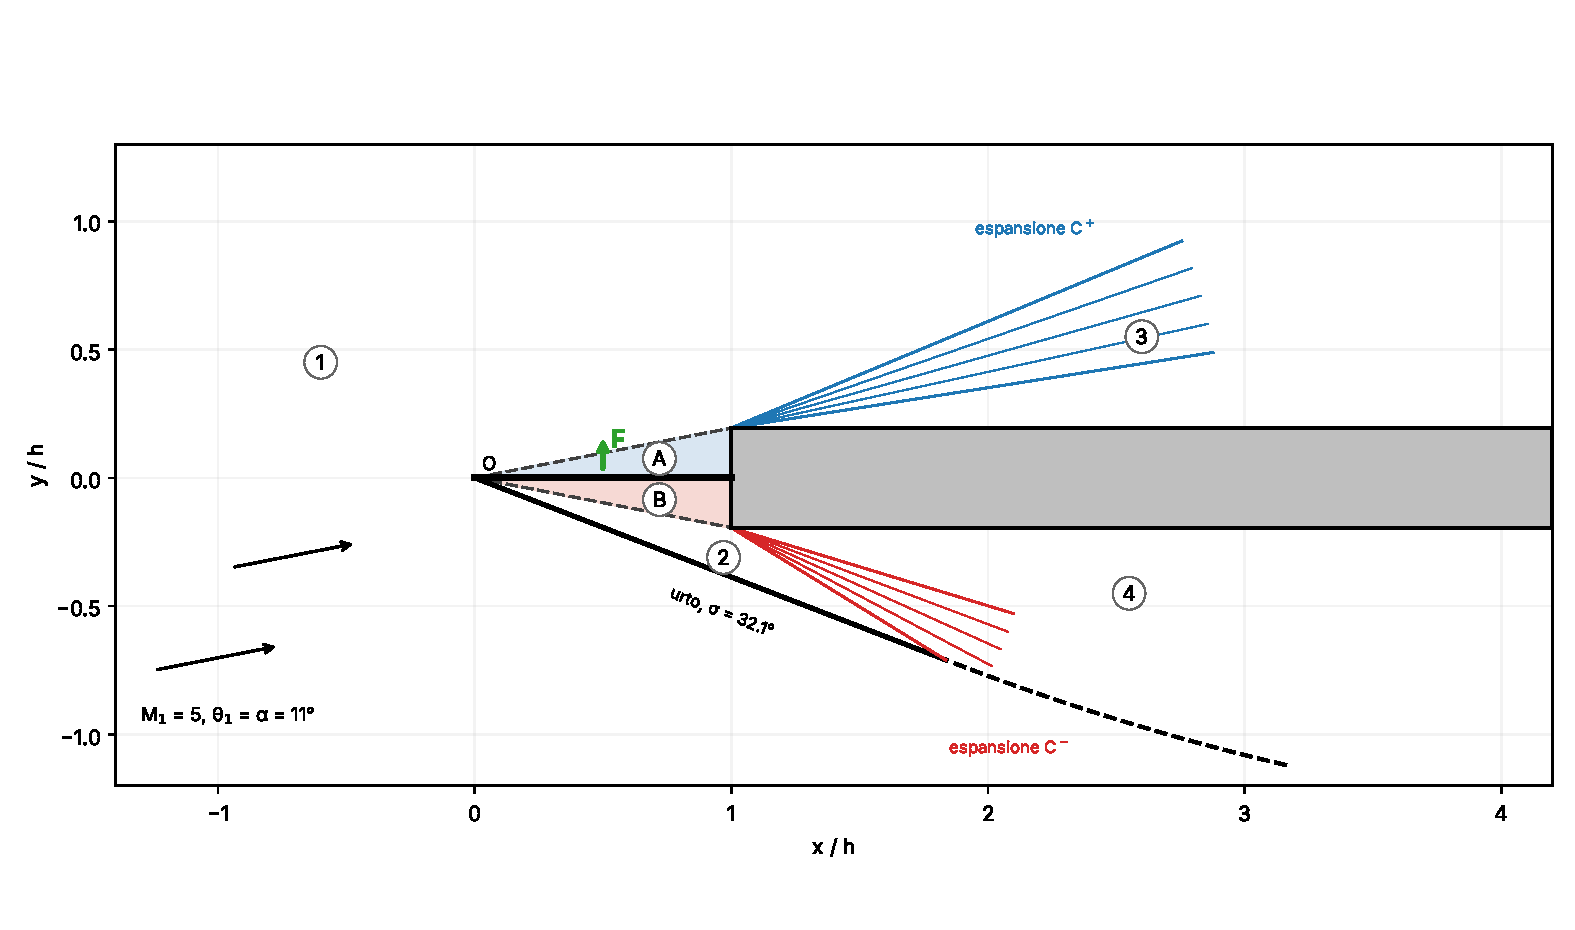
\includegraphics[width=\textwidth]{campo.pdf}
  \caption{Piano fisico in unità di $h$. Segmento in nero spesso, corpo in grigio, bolle A e B colorate, linee di
  scorrimento tratteggiate a $\pm\ang{11}$. Urto da O (nero) che, raggiunto dal ventaglio inferiore, si indebolisce e
  si incurva (tratteggio, qualitativo); ventagli d'espansione agli spigoli in blu ($\Cp$) e rosso ($\Cm$). F è la
  forza sul segmento.}
  \label{fig:campo}
\end{figure}

\begin{table}[H]
  \centering
  \small
  \begin{tabular}{clll}
    \toprule
    Stato & Regione & Onda che lo genera & Natura \\
    \midrule
    1 & corrente indisturbata (anche sopra A) & -- & -- \\
    A & bolla superiore, $p_A=p_1$ & -- & fluido morto \\
    2 & sotto la bolla B, dietro l'urto & urto in O, $\Cm$ & compressione (urto) \\
    B & bolla inferiore, $p_B=p_2$ & -- & fluido morto \\
    3 & sopra il corpo, a valle dello spigolo superiore & ventaglio, $\Cp$ & espansione \\
    4 & sotto il corpo, a valle dello spigolo inferiore & ventaglio, $\Cm$ & espansione \\
    \bottomrule
  \end{tabular}
  \caption{Stati e onde. Sui contorni delle bolle: $p_A=p_1$, $\theta=+\ang{11}$; $p_B=p_2$, $\theta=-\ang{11}$.}
\end{table}

%==============================================================================
\section{Scorciatoie fisiche}
La scelta $b=2h\tan\alpha$ rende il problema quasi immediato: il lato superiore non genera onde, quindi $p_A=p_1$
senza calcoli, e quello inferiore è un solo urto obliquo con deviazione nota, $2\alpha$. Inoltre, essendo la corrente
supersonica, la pressione nelle bolle dipende solo da ciò che avviene fra O e i contorni delle bolle: il campo
attorno al resto del corpo (ventagli agli spigoli, scia) non serve.

%==============================================================================
\section{Calcolo}

\subsection*{a) Bolla superiore A}
Il contorno di A è inclinato di $\arctan\!\left(b/2h\right)=\ang{11}=\theta_1$: deviazione nulla, quindi
\[
p_A=p_1=1 .
\]

\subsection*{b) Urto inferiore: stato 2 e bolla B}
Deviazione $\theta=\theta_1-(-\alpha)=2\alpha=\ang{22}$, famiglia $\Cm$. L'angolo d'urto viene dalle relazioni di
Rankine--Hugoniot applicate alla componente normale. La componente tangenziale si conserva e la portata normale pure:
\[
V_1\cos\sigma=V_2\cos(\sigma-\theta),\qquad \rho_1V_1\sin\sigma=\rho_2V_2\sin(\sigma-\theta)
\ \Rightarrow\ \frac{\tan(\sigma-\theta)}{\tan\sigma}=\frac{\rho_1}{\rho_2}=\frac{(\gamma-1)M_{n1}^2+2}{(\gamma+1)M_{n1}^2},
\]
con $M_{n1}=M_1\sin\sigma$; sviluppando la tangente della differenza si ottiene la relazione $\theta$--$\sigma$--$M$
\[
\tan\theta=2\cot\sigma\,\frac{M_1^2\sin^2\sigma-1}{M_1^2(\gamma+\cos2\sigma)+2}.
\]
Per $M_1=5$ e $\theta=\ang{22}$ la risolvo per tentativi sul ramo debole, partendo dalle tabelle:
\begin{table}[H]
  \centering
  \small
  \begin{tabular}{cc}
    \toprule
    $\sigma$ & $\theta(\sigma)$ \\
    \midrule
    \ang{30} & \ang{20.2} \\
    \ang{32} & \ang{21.9} \\
    \ang{32.1} (interpolato) & \ang{22.0} \\
    \bottomrule
  \end{tabular}
  \caption{Tentativi sull'angolo d'urto.}
\end{table}
\[
\sigma=\ang{32.1},\qquad M_{n1}=M_1\sin\sigma=2{,}66 .
\]
Dalle relazioni dell'urto normale applicate a $M_{n1}$:
\[
\frac{p_2}{p_1}=1+\frac{2\gamma}{\gamma+1}\left(M_{n1}^2-1\right)=8{,}08,\qquad
\frac{\rho_2}{\rho_1}=\frac{(\gamma+1)M_{n1}^2}{(\gamma-1)M_{n1}^2+2}=3{,}51,
\]
\[
M_{n2}^2=\frac{1+\delta M_{n1}^2}{\gamma M_{n1}^2-\delta}\ \Rightarrow\ M_{n2}=0{,}499,\qquad
M_2=\frac{M_{n2}}{\sin(\sigma-\theta)}=2{,}84,
\]
\[
\frac{p_{02}}{p_{01}}=\left[\frac{(\gamma+1)M_{n1}^2}{(\gamma-1)M_{n1}^2+2}\right]^{\frac{\gamma}{\gamma-1}}
\left[\frac{\gamma+1}{2\gamma M_{n1}^2-(\gamma-1)}\right]^{\frac{1}{\gamma-1}}=0{,}438 .
\]
Il fronte dell'urto è inclinato di $\theta_1-\sigma=\ang{-21.1}$ sul segmento. Per la bolla B:
\[
p_B=p_2=8{,}08\,p_1 .
\]

\subsection*{c) Forza sul segmento}
Su ciascuna faccia la pressione è uniforme, quindi per unità di apertura la forza è normale al segmento, diretta
dalla faccia inferiore verso quella superiore, e vale
\[
F=\int_0^h(p_B-p_A)\,dx=(p_2-p_1)\,h=7{,}08\,p_1h,\qquad \frac{F}{q_1h}=\frac{p_2-p_1}{\tfrac{\gamma}{2}p_1M_1^2}=0{,}405 .
\]
Scomposta negli assi della corrente indisturbata (il segmento è inclinato di $\alpha$ sulla corrente):
\[
L=F\cos\alpha=6{,}95\,p_1h\ \ (c_L=0{,}397),\qquad D=F\sin\alpha=1{,}35\,p_1h\ \ (c_D=0{,}077).
\]

\subsection*{d) Spigoli del corpo: stati 3 e 4 (per il quadro del campo)}
Sopra, ventaglio $\Cp$ ($\theta+\nu$ costante) da $\theta_1=\ang{11}$ a $\theta_3=0$:
\[
\nu_3=\nu_1+(\theta_1-\theta_3)=\ang{87.9}\ \Rightarrow\ M_3=6{,}46,\qquad
p_3=p_1\left(\frac{1+\delta M_1^2}{1+\delta M_3^2}\right)^{\frac{\gamma}{\gamma-1}}=0{,}212 .
\]
Sotto, ventaglio $\Cm$ ($\theta-\nu$ costante) da $\theta_2=\ang{-11}$ a $\theta_4=0$:
\[
\nu_4=\nu_2+(\theta_4-\theta_2)=\ang{57.5}\ \Rightarrow\ M_4=3{,}44,\qquad
p_4=p_2\left(\frac{1+\delta M_2^2}{1+\delta M_4^2}\right)^{\frac{\gamma}{\gamma-1}}=3{,}33 .
\]
La testa del ventaglio inferiore ($\theta_2-\mu_2=\ang{-31.6}$) è più inclinata dell'urto e lo raggiunge a
$x\approx1{,}8\,h$: da lì l'urto si indebolisce e si incurva. Avviene tutto a valle delle bolle.

%==============================================================================
\section{Verifiche a posteriori}
\begin{itemize}
\item Geometria del cuneo equivalente: $b/2h=\tan\ang{11}$ a cinque cifre, contorno di A parallelo alla corrente.
  \emph{Verificata.}
\item Urto attaccato: $\ang{22}<\theta_{\max}(5)=\ang{41.1}$. \emph{Verificata.}
\item Ramo debole: $\sigma=\ang{32.1}$, minore di \ang{66.6} (angolo d'urto della deviazione massima); il ramo forte ($\sigma=\ang{83.9}$)
  richiederebbe una contropressione che una corrente esterna non ha. \emph{Scartato il forte.}
\item Urto di compressione, entropia crescente: $M_{n1}=2{,}66>1$, $p_{02}/p_{01}=0{,}438<1$. \emph{Verificata.}
\item Regioni esterne supersoniche: $M_2=2{,}84$, $M_3=6{,}46$, $M_4=3{,}44$, quindi il modello 2D stazionario
  supersonico è lecito. \emph{Verificata.}
\item L'urto passa sotto la bolla e il corpo: in $x=h$ sta a $y=-0{,}387\,h$, sotto lo spigolo ($-0{,}194\,h$).
  \emph{Verificata.}
\item Onde agli spigoli: entrambe espansioni, a valle delle bolle, senza effetto su $p_A$ e $p_B$. \emph{Verificata.}
\end{itemize}

%==============================================================================
\section{Risultati}
\begin{table}[H]
  \centering
  \begin{tabular}{lll}
    \toprule
    Grandezza & Valore & Esatto / approssimato \\
    \midrule
    $p_A$ (faccia superiore) & $p_1$ & esatto nel modello \\
    $p_B$ (faccia inferiore) & $8{,}08\,p_1$ & esatto nel modello \\
    angolo d'urto, $M_2$ & \ang{32.1}, $2{,}84$ & esatto \\
    $F$ (normale al segmento, verso l'alto) & $7{,}08\,p_1h=0{,}405\,q_1h$ & esatto nel modello \\
    $L$, $D$ (assi della corrente) & $6{,}95\,p_1h$, $1{,}35\,p_1h$ & esatto nel modello \\
    \bottomrule
  \end{tabular}
  \caption{Risultati per unità di apertura. ``Esatto nel modello'': esatto una volta accettato lo schema delle bolle
  di fluido morto.}
\end{table}

%==============================================================================
\section{Rappresentazioni}
\begin{figure}[H]
  \centering
  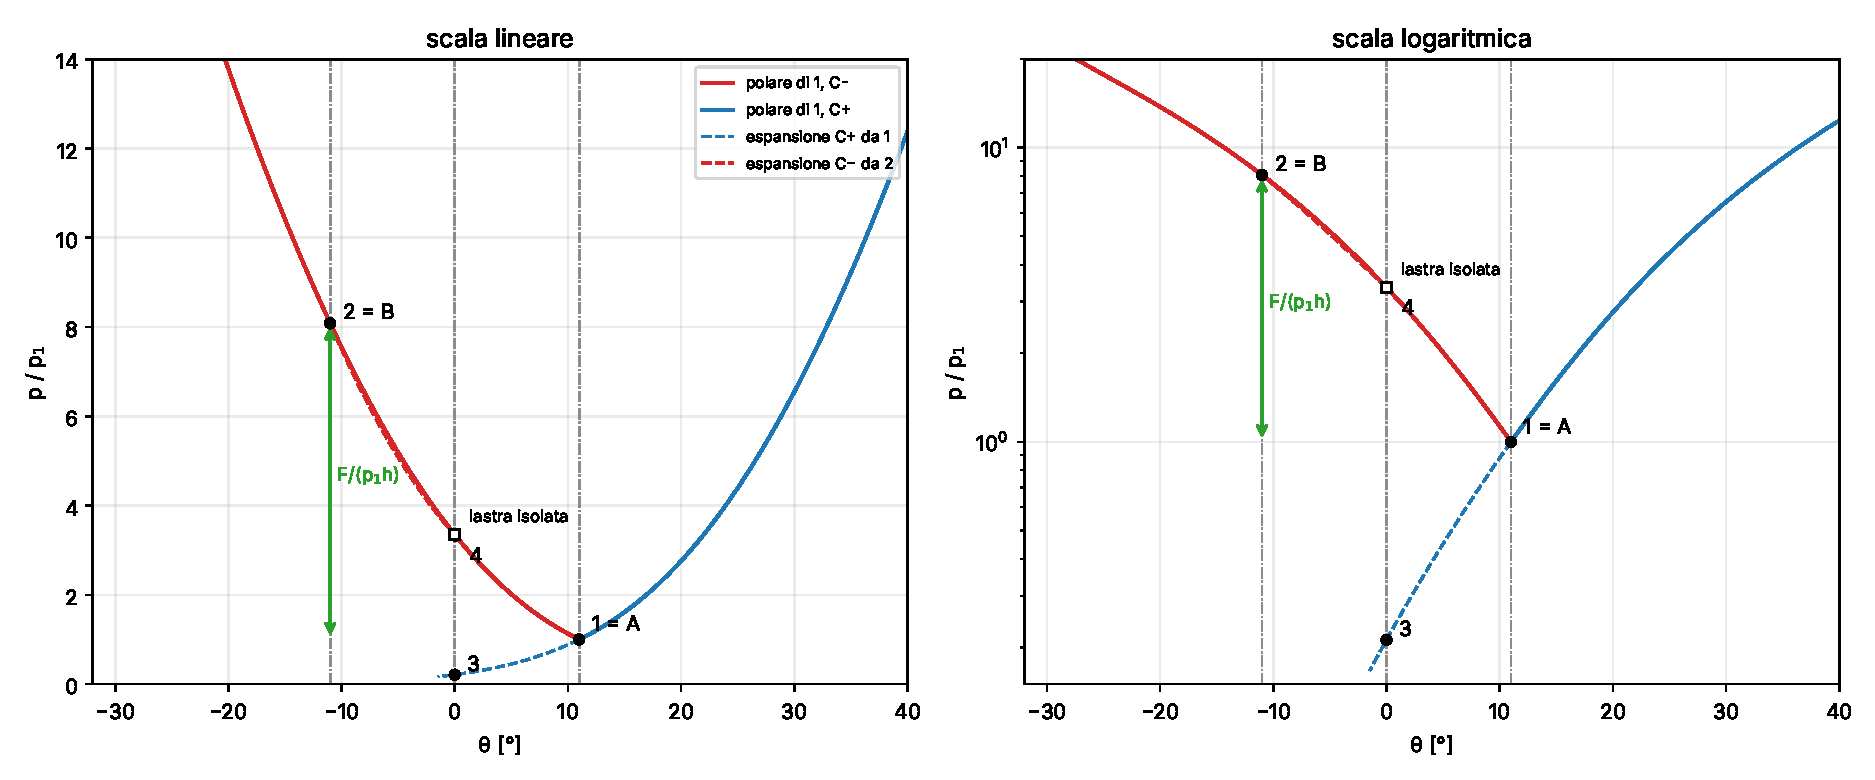
\includegraphics[width=\textwidth]{p_theta.pdf}
  \caption{Piano $p$--$\theta$ in scala lineare (sinistra) e logaritmica (destra): polare di 1 ($\Cm$ rossa, $\Cp$
  blu, ramo debole; il ramo forte è fuori scala), espansioni tratteggiate. Rette verticali: contorni delle bolle
  ($\pm\ang{11}$) e pareti ($\theta=0$). Il quadratino è la faccia inferiore della lastra isolata.}
  \label{fig:pt}
\end{figure}
La polare di 1 parte dal punto $(\ang{11},1)$, non dall'origine. Il contorno di A coincide con $\theta_1$, quindi lo
stato di A è il punto 1 stesso. Il contorno di B taglia il ramo $\Cm$ della polare in 2: il segmento verde fra 1 e 2
è proprio $F/(p_1h)$. Dagli stati 1 e 2 le espansioni agli spigoli portano a 3 e 4 su $\theta=0$. Lo stato 4 ha
quasi la stessa pressione della faccia inferiore della lastra isolata (3,33 contro 3,35), ma vi arriva con un urto
più forte seguito da un'espansione, quindi con pressione totale molto minore.

Le pressioni vanno da 0,21 a 8,1. La scala lineare mostra in proporzione il carico, cioè la distanza fra 1 e 2, e la
ripidità della polare a $M=5$. La scala logaritmica separa gli stati a bassa pressione (3, 1) e mostra i rapporti
di pressione: l'espansione di \ang{11} riduce la pressione di quasi 5 volte, l'urto di \ang{22} la aumenta di 8;
deforma però la concavità della polare.

\begin{figure}[H]
  \centering
  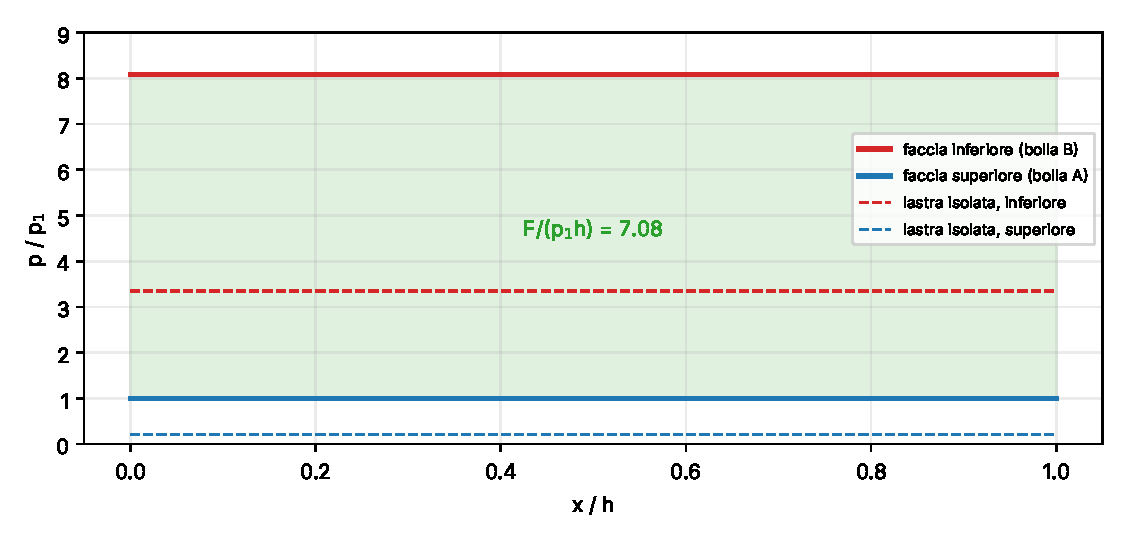
\includegraphics[width=0.72\textwidth]{carico.pdf}
  \caption{Pressione sulle due facce del segmento: con il corpo (continue) e per la lastra isolata alla stessa
  incidenza (tratteggiate). L'area verde è il carico $F/(p_1h)$.}
  \label{fig:carico}
\end{figure}
Il carico è uniforme lungo il segmento: le due facce vedono ciascuna una bolla a pressione costante. Le linee
tratteggiate mostrano cosa cambia senza il corpo: la faccia inferiore scenderebbe a 3,35 e quella superiore a 0,21.

%==============================================================================
\section{Discussione fisica}
\textbf{Il corpo comanda il carico sul segmento.} Il segmento non vede direttamente la corrente: ciascuna faccia
sta in una bolla la cui pressione è fissata dal cuneo equivalente. Per la lastra isolata alla stessa incidenza
(urto di \ang{11} sotto, espansione di \ang{11} sopra) si avrebbe $F=(3{,}35-0{,}21)\,p_1h=3{,}14\,p_1h$, cioè
$0{,}179\,q_1h$. Con il corpo il carico è 2,3 volte maggiore. La faccia inferiore guadagna molto perché l'urto devia
la corrente di \ang{22} invece di \ang{11}; la faccia superiore perde l'aspirazione dell'espansione e torna a $p_1$,
ma questa perdita (0,8) è molto minore del guadagno sotto (4,7).

\textbf{Direzione.} Senza attrito e con spessore nullo la forza è normale al segmento. Negli assi della corrente
la resistenza è $F\sin\alpha$, appena un quinto della portanza: sul segmento la resistenza viene tutta
dall'inclinazione. La resistenza del corpo intero, con le facce frontali alle pressioni $p_1$ e $p_2$ e la base, è
un'altra cosa e non è richiesta.

\textbf{Limiti del modello.} Senza separazione il problema non avrebbe soluzione nel modello 2D supersonico: davanti
alle facce frontali si staccherebbero urti curvi con regioni subsoniche, e il campo non si calcolerebbe con urti
obliqui e polari. Lo schema delle bolle è quello dei corpi con l'ago, ed è il solo coerente con il dato
$b=2h\tan\alpha$; resta un'idealizzazione. Nella realtà la separazione può avvenire un po' a valle dello
spigolo, la pressione nella bolla non è perfettamente uniforme e lo strato di scorrimento, riattaccandosi allo
spigolo, produce una piccola ricompressione locale. Il risultato va quindi letto come il valore del modello a
fluido morto, che coglie l'effetto principale: un segmento sottile davanti a un corpo tozzo si comporta come il
vertice di un cuneo.

\end{document}
